% Drawing 154/04-5 -- folder 154, batch 04, archive page 71 (PDF page 72).
% Transcription: figures, en haut de la colonne de droite : un disque au bord vert clair traversé de deux pseudo-droites rouges qui se croisent près du haut et du bas, des arcs épais noirs marqués $a'$ et $a$ ; une droite au crayon le traverse et touche un second disque esquissé au crayon. Au-dessous, un disque au bord vert foncé, deux pseudo-droites rouges se croisant en haut et en bas, entourées de petits arcs vert foncé et vert clair, avec des arcs épais noirs marqués $b^{\ast}$, $a'$ en haut, $b'$, $b$ et $a$ en bas. La dernière ligne de la page est écrite sous une ligne raturée
% Kind: disks with two pseudolines crossing near top and bottom; arcs a, a', b, b', b*. Method 2 (schematic redraw from the facsimile). Status: ok.
% Notes: Top of the right column: a disk with a light green rim crossed by two red pseudolines crossing near the top and the bottom, thick black arcs marked a' and a; a pencil line crosses it and touches a second disk sketched in pencil (a second pencil line crosses that one). Below: a disk with a dark green rim, two red pseudolines crossing at the top and the bottom, surrounded by small arcs in light green (top) and dark green (bottom), with thick black arcs marked b*, a' at the top and b', b and a at the bottom. The small figure in the left column (a pencil of lines on a green line) is not covered by this mark. Read from the page view.
% Coordinates: 1 unit = 1 mm = 1/100 of the crop width (bbox in page fractions: [0.569, 0.092, 0.873, 0.339]).
% Redrawn by Claude (claude-opus-5-5), issue #73, 2026-11-07; not checked by a human; not compiled (no TeX in the session).
% Rights: reproduces part of the work -- behind RENDER_TRANSCRIPTS, never published by itself.
\documentclass[tikz,border=3pt]{standalone}
\usepackage{amsmath,amssymb}
\usetikzlibrary{patterns,arrows.meta}
\tikzset{Or/.style={orange!90!black}, Ye/.style={yellow!80!orange}, Lg/.style={green!60!black!70}, Dg/.style={green!45!black}, Br/.style={brown!80!black}, Rd/.style={red!85!black}, Bl/.style={blue!70!black}, Gy/.style={black!40}, pencil/.style={black!45}, struck/.style={black!35}, mark/.style={circle,draw,inner sep=1.3pt}, pt/.style={circle,fill,inner sep=0.9pt}, opt/.style={circle,draw,fill=white,inner sep=1.1pt}}
\begin{document}
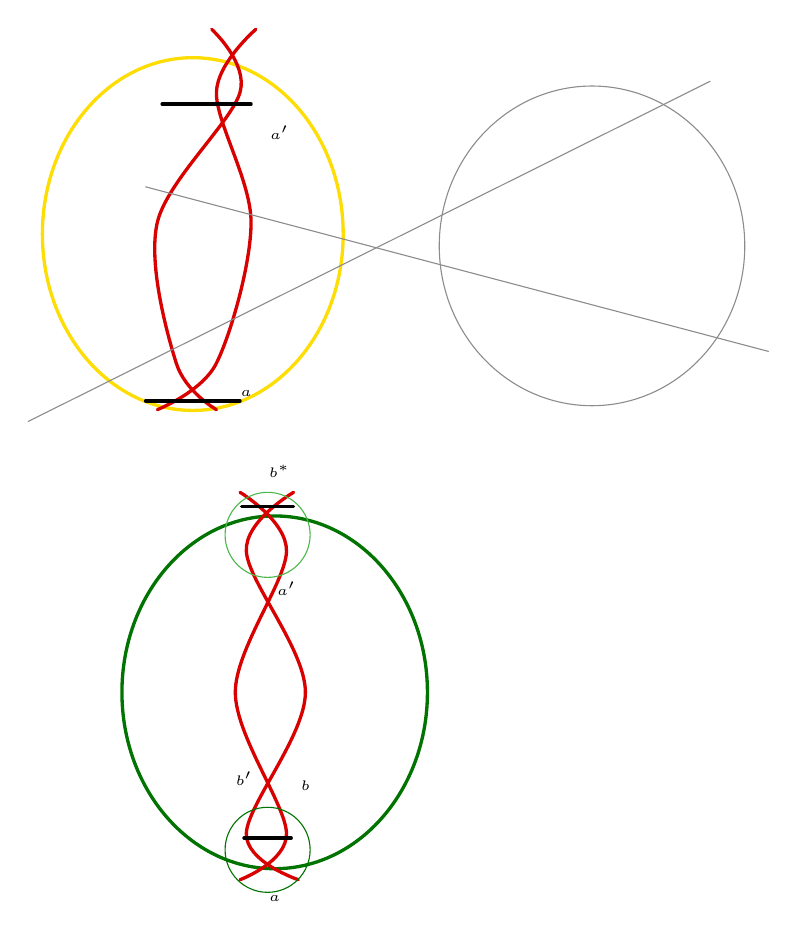
\begin{tikzpicture}[x=1mm,y=1mm,line cap=round,line join=round,font=\scriptsize]
\draw[Ye,very thick] (23.9,-28.4) ellipse[x radius=19.1, y radius=22.4];
\draw[Rd,very thick] plot[smooth, tension=0.55] coordinates {(26.3,-2.4) (29.9,-10.4) (19.4,-26.9) (21.8,-44.8) (26.9,-50.7)};
\draw[Rd,very thick] plot[smooth, tension=0.55] coordinates {(31.9,-2.4) (26.9,-10.4) (31.3,-26.9) (26.9,-44.8) (19.4,-50.7)};
\draw[very thick] (20,-11.9) -- (31.3,-11.9);
\node[inner sep=1pt] at (34.9,-15.5) {\tiny $a'$};
\draw[very thick] (17.9,-49.6) -- (29.9,-49.6);
\node[inner sep=1pt] at (30.7,-48.7) {\tiny $a$};
\draw[pencil] (3,-52.2) -- (89.6,-9);
\draw[pencil] (17.9,-22.4) -- (97,-43.3);
\draw[pencil] (74.6,-29.9) ellipse[x radius=19.4, y radius=20.3];
\draw[Dg,very thick] (34.3,-86.6) ellipse[x radius=19.4, y radius=22.4];
\draw[Rd,very thick] plot[smooth, tension=0.55] coordinates {(29.9,-61.2) (35.8,-68.7) (29.3,-86.6) (35.8,-104.5) (29.9,-110.4)};
\draw[Rd,very thick] plot[smooth, tension=0.55] coordinates {(36.7,-61.2) (30.7,-68.7) (38.2,-86.6) (30.7,-104.5) (37.3,-110.4)};
\draw[Lg] (33.4,-66.6) circle[radius=5.4];
\draw[Dg] (33.4,-106.6) circle[radius=5.4];
\draw[very thick] (30.1,-63) -- (36.7,-63);
\draw[very thick] (30.4,-105.1) -- (36.4,-105.1);
\node[inner sep=1pt] at (34.9,-58.5) {\tiny $b^{*}$};
\node[inner sep=1pt] at (35.8,-73.4) {\tiny $a'$};
\node[inner sep=1pt] at (30.4,-97.6) {\tiny $b'$};
\node[inner sep=1pt] at (38.2,-98.5) {\tiny $b$};
\node[inner sep=1pt] at (34.3,-112.8) {\tiny $a$};
\end{tikzpicture}
\end{document}
